\documentclass{article}

\usepackage{amsmath}
\usepackage{amssymb}
\usepackage{graphicx}

\usepackage[justification=centering]{caption}
\usepackage[font=footnotesize]{caption}

\newcommand{\noi}{\noindent}

\begin{document}

\begin{section}{Elevator Pitch}
TURF is NOMINATE for elections. The goal of the project is to place candidates and counties in ideology space based only on county-level election results.

The underlying mathematical model assumes that voters have a position in ideology space, and that candidates have both a position in ideology space and a scalar ``strength'' which captures, essentially, what would be impacted by a good or bad debate performance, or an ad buy. Given a choice of positions and strengths, TURF predicts election results at the county level. The computational challenge is to identify the choice of positions and strengths that most accurately predicts a given set of real-world election results.

As with NOMINATE, all ``qualitative'' analysis---e.g.\ the significance of the axes---occurs post-hoc. If successfully implemented, TURF would help answer a number of questions of high importance in the field of political science (here framed in the context of American elections). To name a few:
\begin{itemize}
\item What are the primary components of voter ideology? Are the the similar to those of legislator ideology?
\item How did Donald Trump win the 2016 Republican Primary? Could it have gone differently?
\item How has the ideology of voters and candidates shifted over time? When were there significant party realignments?
\item For a given electorate and set of candidates, what is the expected election result?
\end{itemize}
\noi It seems that much of the use of TURF would be ``retrospective,'' that is, analyzing elections which have already occurred. However, there is predictive potential---with sufficient data, TURF is essentially an election forecast model without polls.
\end{section}

\begin{section}{Mathematical Model}

A \textbf{voter} $V$ has a \textbf{position} $(x,y)$ in ideological space $\mathbb{R}^2$. \\

\noi A \textbf{candidate} $K$ has a \textbf{stance} $(p,q) \in \mathbb{R}^2$ and a scalar \textbf{strength} $s_K$. Strength intends to capture the relative electoral appeal of the candidate, influenced by name recognition and favorability. \\

\noi The \textbf{distance} $d(V, K)$ between a voter $V$ and a candidate $K$ is the Euclidean distance between $(x,y)$ and $(p,q)$. Distance is a measure of the ideological distance between the voter and the candidate. \\

\noi The \textbf{salience} $c_K(V)$ of a candidate $K$ to a voter $V$ is given by $$c_K(V) = \frac{s_K}{d(V, K) + 1}$$

\noi Salience represents, more or less, how desirable a candidate is to a voter. For a given voter, a stronger candidate is more salient, all else held equal, and an ideologically closer candidate is more salient, all else held equal. The maximum salience for a candidate $K$ is the strength $s_K$ of that candidate; this maximum is attained for a voter whose position is identical to the stance of the candidate. We expect a voter to vote for whichever candidate is most salient to her.

For a fixed candidate $K$, we can plot $c_K(V)$ in 3-space with $V$ on the $x,y$-plane and $c$ on the $z$-axis. The graph is a harmonic distribution with a central spike of height $s_K$ at the stance of $K$. Plotting this ``salience hill'' for multiple candidates on the same axes, as in Figure 1, reveals the regions of ideological space in which a given candidate is the most salient. \\

\begin{figure}[!h]
\centering
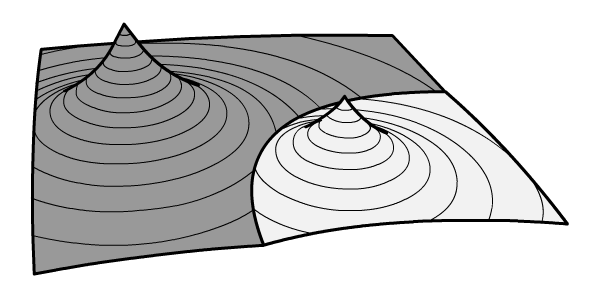
\includegraphics[width=0.5\textwidth]{salience_plot.png}
\caption{Salience plot on $[0,5]\times[0,5]$ for two hypothetical candidates:\newline $K_1$ at $(1,2)$ with strength 4, $K_2$ at $(3,1)$ with strength 3.}
\end{figure}

\noi We use the term \textbf{field} to describe a set $F = \{K_1, \ldots, K_n\}$ of candidates who are competing for voters in a single election. \\

\noi Given a field $F$ of candidates, the \textbf{turf} of a candidate $K \in F$ is the set of all points $(x,y) \in \mathbb{R}^2$ for which a voter $V$ with position $(x,y)$ satisfies $$c_K(V) \ge c_{K'}(V) \text{ for all } K' \in F$$

\noi That is, a candidate's turf is the region in ideological space in which she is the most salient candidate among the field. In a hypothetical scenario where the electorate is uniformly distributed through a finite region in ideology space, a candidate's portion of the vote would be proportional to the area of her turf.

\end{section}
\begin{section}{Justification}

The definition of salience, which is the only ``arbitrary'' theoretical decision made thus far, is chosen so that turf plots (bird's eye views of salience plots) reflect real-world expectations. Here are a few sanity conditions that this model satisfies:
\begin{itemize}
\item The line segment connecting two candidates crosses the boundary between these candidates' turfs; the exact location of this boundary depends on the relative strengths of the candidates.
\item If a candidate's strength increases (through media coverage, perhaps), her turf expands at the margins, with new voters coming from those ``centrist'' regions where her salience was close to that of another candidate.
\begin{figure}[!h]
\centering
\raisebox{-.5\height}{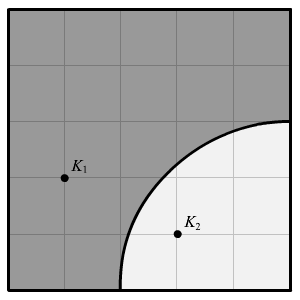
\includegraphics[width=0.3\textwidth]{turf_plot1.png}} $\rightarrow$
\raisebox{-.5\height}{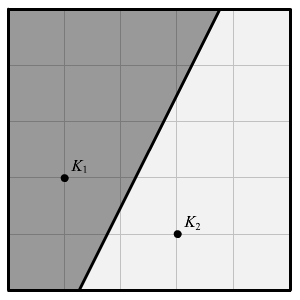
\includegraphics[width=0.3\textwidth]{turf_plot2.png}} $\rightarrow$
\raisebox{-.5\height}{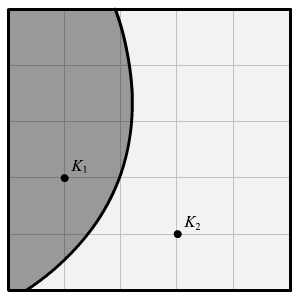
\includegraphics[width=0.3\textwidth]{turf_plot3.png}}
\caption{Turf plot of Figure 1. Strength of $K_2$ increases from 3 to 4 to 5.}
\end{figure}
\item If a candidate's stance shifts, the contours of her turf recenter around her new stance. A weaker candidate benefits from being ideologically heterodox or else she will lose support to a nearby opponent.
\begin{figure}[!h]
\raisebox{-.5\height}{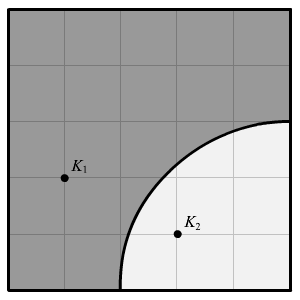
\includegraphics[width=0.3\textwidth]{turf_plot1.png}} $\rightarrow$
\raisebox{-.5\height}{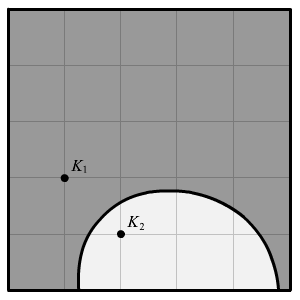
\includegraphics[width=0.3\textwidth]{turf_plot4.png}} $\rightarrow$
\raisebox{-.5\height}{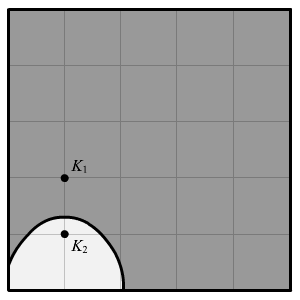
\includegraphics[width=0.3\textwidth]{turf_plot5.png}}
\caption{Turf plot of Figure 1. Stance of $K_2$ moves from $(3,1)$ to $(2,1)$ to $(1,1)$.}
\end{figure}
\item In a field with a large number of candidates, ideologically similar candidates will be punished, allowing for a heterodox candidate to win the greatest support even if she is not preferred in head-to-head matchups.
\item A relatively weak candidate can still gain significant support if her stance lies in an ``unclaimed'' region of ideology space---that is, a region where many voters but few or no candidates exist.
\end{itemize}

\end{section}

\begin{section}{Deriving Ideology from Real-World Data}

\begin{subsection}{Discussion and Limitations}

The TURF model described above provides a theoretical framework for analyzing elections. The challenge now is to describe a mathematical process which takes real-world voting data and ``discovers'' the underlying candidate strengths and stances and the distribution of voter ideology which led to this data.

To do this, we will make a simplifying assumption which is not quite reflective of the real world. We will assume that each county---broadly defined as an administrative level at which voting data is available---is a single point in ideology space, rather than a distribution of points representing individual voters. We will further assume that the portion of the vote a candidate receives in a county is proportional to the salience of that candidate to that county.

The limitations of this approach are apparent if we consider a county with 100 leftist voters and 100 rightist voters, voting in an election with a leftist candidate, a rightist candidate, and a centrist candidate. Since our model will consider this county to exist at the midpoint of its partisan voters, it will likely predict a first-place finish for the centrist candidate when in reality we might expect the centrist to finish third.

This concern can be assuaged if we use ``county'' delimiters that take into account more politically relevant factors than just geography. For instance, we could imagine a later iteration of this model for which ``college-educated, Catholic, Hispanic women aged 30-39 in Queens county" replaces ``all voters in Queens county'' as the level of analysis. In any case, there will be a level of approximation, but to the extent that demographic variables are correlated with vote preference, we can steadily improve the model's accuracy.

\end{subsection}

\begin{subsection}{Mathematical Specification of Optimal Arrangement}

For a field $F = \{K_1, \ldots, K_n\}$, we define the \textbf{predicted vote results} $\{r_1, \ldots, r_n\}$ in a county $T$ as follows:

$$r_i(T) = \frac{c_{K_i}(T)}{ \sum_{j=1}^n c_{K_j}(T)}$$

\noi The predicted vote results in a county sum to 1 and are each proportional to the salience of the corresponding candidate to that county.

Given a real-world field of candidates and set of counties, an accurate model of candidate stances and voter positions would produce predicted vote results in each county that approximately reflect the actual vote results in that county. For the hypothetical case in which a large number of counties simultaneously hold elections, we now provide a mathematical description of optimal candidate stances, candidate strengths, and county positions so as to minimize the error between predicted and actual vote results. \\

\noi A \textbf{county measurement} on a county $T$ among a field $F = \{K_1, \ldots, K_n\}$ is a map $\mu : K_i \mapsto a_i$ which satisfies $\sum_{i=1}^n a_i = 1$. These $a_i$ are the \textbf{actual vote results} in $T$. County measurements are given by real-world data from elections in which voters in a county each choose between a field of candidates. \\

\noi Given a county $T$, a field $F = \{K_1, \ldots, K_n\}$, and a measurement $\mu$, the \textbf{county prediction error (CPE)} is the mean squared error between the predicted vote results and actual vote results in $T$. That is:

$$\text{CPE} = \frac{1}{n} \sum_{i=1}^n (r_i - a_i)^2$$

\noi We use the term \textbf{electorate} to describe a set $E = \{T_1, \ldots, T_m\}$ of counties who choose between the same field of candidates in a single election. \\

\noi A \textbf{simultaneous electorate measurement (SEM)} on an electorate $E = \{T_1, \ldots, T_m\}$ among a field $F$ is a set $\{\mu_1, \ldots, \mu_m\}$ for which each $\mu_i$ is a county measurement on $T_i$ among $F$. SEMs are given by real-world data from elections in which voters in multiple counties, voting on the same day, each choose between a field of candidates. \\

\noi Given an electorate $E = \{T_1, \ldots, T_m\}$, a field $F$, and a SEM $\{\mu_1, \ldots, \mu_m\}$ on $E$ among $F$, the \textbf{electorate prediction error} is the sum of the county prediction errors for each county in $E$. That is:

$$\text{EPE} = \sum_{i=1}^m \text{CPE}(T_i, F, \mu_i)$$

\noi This is a measure of how ``far off'' our candidate stances, candidate strengths, and voter positions are.

Given a SEM, we may allow candidate stances, candidate strengths, and voter positions to vary, calculating the EPE for each arrangement of counties and candidates. We choose the electorate $E^*$ and field $F^*$ which minimize EPE for the given SEM; this is the \textbf{optimal arrangement} for this SEM. Using real-world election data for our SEM, the optimal arrangement gives an approximate ideological map of counties and candidates which explains voter behavior.

Developing an algorithm which, given actual vote results, locates this optimal arrangement is non-trivial. Our attempts thus far to develop and implement such an algorithm are covered in ``02.implementation'' in this directory.

\end{subsection}

\end{section}

\begin{section}{Further Theoretical Work}

There are numerous extensions of the above theoretical framework which would increase the explanatory and predictive power of TURF. Below are a few purely theoretical problems which we intend to solve.

\begin{subsection}{Staggered Measurement}

In real-world situations, we might have county-level data from elections that took place at different times; for example, presidential primaries in the United States are staggered over the course of several months. In this time, candidates may drop out or gain appeal, which adversely impacts our results. Any county voting after a candidate $K$ suspended her campaign would be positioned far away from the stance of $K$, even if it were nearly identical in ideological leanings to a similar county which voted before $K$ dropped out.

To account for this complication, we will replace the constant $s_K$ with a function $s_K(t)$ that varies over time, and we will associate each measurement with a time at which it was taken.

If we develop a model which successfully backs out these $s(t)$ functions, this will be an explanatory feat---the strength functions are the core ``narrative'' of the race. They may move up and down in response to debate performances, ad campaigns, gaffes, and so forth. The media at present reports on the county measurements, which are very noisy as a result of the ideological diversity of counties; we should be more interested in the changes in strength.

To do this, we need to develop an adjusted definition of EPE which incorporates some appropriate ``punishment'' for $s(t)$ functions which move ``too fast,'' so as to avoid solutions which minimize EPE by assigning each candidate a $s(t)$ proportional to her vote percentage of all counties voting at time $t$.

\end{subsection}

\begin{subsection}{Assigning Axes}

Once we have the map of counties in $\mathbb{R}^2$, we can identify what the axes ``mean'' by correlating directions in ideology space with external variables about the candidates or counties.

\end{subsection}

\begin{subsection}{Field Splicing}

For the specific case of U.S.\ presidential elections, there are only two candidates in the general election, which greatly limits the applicability of TURF. However, multi-candidate primary elections provide information about county and candidate ideology. Given optimal arrangements for two cases of staggered measurement (in this case, the Republican and Democratic primaries) we need to develop a process for ``splicing" these maps together into one coherent idelogical map of the United States.

\end{subsection}

\begin{subsection}{Historical Splicing}

TURF gains additional explanatory power if we are able to view the ideological distribution of candidates and counties not just in one election but over a timeseries of elections. We need to develop a process for ``splicing'' the results of individual elections onto a fixed set of ideological axes, with each county moving as little as possible between elections.

\end{subsection}

\end{section}

\end{document}